%
% Niniejszy plik stanowi przykład formatowania pracy magisterskiej na
% Wydziale MIM UW.  Szkielet użytych poleceń można wykorzystywać do
% woli, np. formatujac wlasna prace.
%
% Zawartosc merytoryczna stanowi oryginalnosiagniecie
% naukowosciowe Marcina Wolinskiego.  Wszelkie prawa zastrzeżone.
%
% Copyright (c) 2001 by Marcin Woliński <M.Wolinski@gust.org.pl>
% Poprawki spowodowane zmianami przepisów - Marcin Szczuka, 1.10.2004
% Poprawki spowodowane zmianami przepisow i ujednolicenie 
% - Seweryn Karłowicz, 05.05.2006
% dodaj opcję [licencjacka] dla pracy licencjackiej
\documentclass{pracamgr}

\usepackage{polski}

%Jesli uzywasz kodowania polskich znakow ISO-8859-2 nastepna linia powinna byc 
%odkomentowana
%\usepackage[latin2]{inputenc}
%Jesli uzywasz kodowania polskich znakow CP-1250 to ta linia powinna byc 
%odkomentowana
\usepackage[utf8]{inputenc}
\RequirePackage{graphicx}
\RequirePackage{longtable}

\newcommand{\emptyP}{\mbox{$\epsilon$}}
\newcommand{\terminal}[1]{\mbox{{\texttt {#1}}}}
\newcommand{\nonterminal}[1]{\mbox{$\langle \mbox{{\sl #1 }} \! \rangle$}}
\newcommand{\arrow}{\mbox{::=}}
\newcommand{\delimit}{\mbox{$|$}}
\newcommand{\reserved}[1]{\mbox{{\texttt {#1}}}}
\newcommand{\literal}[1]{\mbox{{\texttt {#1}}}}
\newcommand{\symb}[1]{\mbox{{\texttt {#1}}}}
% Dane magistranta:

\author{Imię i nazwisko}

\nralbumu{nralbumu}

\title{Intuicyjny język wyszukiwania TQL (Tablets Query Language)}

\tytulang{Intuitive query language TQL (Tablets Query Language)}

%kierunek: Matematyka, Informatyka, ...
\kierunek{Informatyka}

% informatyka - nie okreslamy zakresu (opcja zakomentowana)
% matematyka - zakres moze pozostac nieokreslony,
% a jesli ma byc okreslony dla pracy mgr,
% to przyjmuje jedna z wartosci:
% {metod matematycznych w finansach}
% {metod matematycznych w ubezpieczeniach}
% {matematyki stosowanej}
% {nauczania matematyki}
% Dla pracy licencjackiej mamy natomiast
% mozliwosc wpisania takiej wartosci zakresu:
% {Jednoczesnych Studiow Ekonomiczno--Matematycznych}

% \zakres{Tu wpisac, jesli trzeba, jedna z opcji podanych wyzej}

% Praca wykonana pod kierunkiem:
% (podać tytuł/stopień imię i nazwisko opiekuna
% Instytut
% ew. Wydział ew. Uczelnia (jeżeli nie MIM UW))
\opiekun{dra Roberta Dąbrowskiego\\
  Instytut Informatyki\\
  }

% miesiąc i~rok:
\date{czerwiec 2010}

%Podać dziedzinę wg klasyfikacji Socrates-Erasmus:
\dziedzina{ 
%11.0 Matematyka, Informatyka:\\ 
%11.1 Matematyka\\ 
%11.2 Statystyka\\ 
11.3 Informatyka\\ 
%11.4 Sztuczna inteligencja\\ 
%11.5 Nauki aktuarialne\\
%11.9 Inne nauki matematyczne i informatyczne
}

%Klasyfikacja tematyczna wedlug AMS (matematyka) lub ACM (informatyka)
\klasyfikacja{H. INFORMATION SYSTEMS\\
H.2. DATABASE MANAGEMENT\\
H.2.3 Languages}

% Słowa kluczowe:
\keywords{}

% Tu jest dobre miejsce na Twoje własne makra i~środowiska:
\newtheorem{defi}{Definicja}[section]

% koniec definicji

\begin{document}
\maketitle

%tu idzie streszczenie na strone poczatkowa
\begin{abstract}
Sumerologia jest dziedziną badań nad antycznym językiem Sumerów, w której
kluczowym zagadnieniem jest przeszukiwanie dużych zbiorów informacji
zapisanych na odnalezionych tabliczkach sumeryjskich.

W pracy przedstawiono definicję przeznaczonego dla sumerologów intuicyjnego
języka przeszukiwania zbiorów tabliczek (Tablets Query Language) wraz z jego
przykładową implementacją opartą na relacyjnej bazie danych.

%TODO: drugi intuicyjny
Celem tej pracy jest stworzenie języka zapytań intuicyjnego dla sumerologów,
stanowiącego znaczące uproszczenie w stosunku do SQL dzięki wprowadzeniu pojęć 
naturalnych dla rozważanej dziedziny. Jednocześnie TQL nadal
pozwala na tworzenie skomplikowanych zapytań wyszukujących, natomiast nie 
udostępnia funkcji tworzących i modyfikujących bazę. Można go rozszerzać 
i zmieniać tak, by mógł służyć też do innych zastosowań.
\end{abstract}

\tableofcontents
%\listoffigures
%\listoftables

\chapter*{Wprowadzenie}
\addcontentsline{toc}{chapter}{Wprowadzenie}

\ \ \ \ Sumerolodzy posiadają bazę danych składającą się z prawie 50 tys. tabliczek sumeryjskich w wersji elektronicznej. Potrzebują prostego i intuicyjnego języka służącego do ich wyszukiwania, który jak najmniej będzie ograniczał siłę wyrazu, a jego wykorzystanie będzie powodowało jak najmniejszy narzut czasowy.

  Istnieją też inne grupy ludzi potrzebujące podobnego języka (np. językoznawcy). Większość programów ułatwiających tworzenie zapytań jest skomplikowana, daje ograniczone możliwości lub jest przystosowana głównie do przetwarzania danych liczbowych. Tablets Query Language rozwiązuje te problemy: jest prosty i intuicyjny, przystosowany głównie do tekstów, minimalnie zmniejsza siłę wyrazu oraz łatwo go rozbudowywać. 

  Język TQL jest nakładką na inne języki (m.in. SQL). Dla każdego z nich, w zależności od reprezentacji danych, należy skonstruować translator, którego zadaniem będzie przetłumaczenie zapytania. W ramach niniejszej pracy przedstawione zostaną dwa przykładowe translatory.

\chapter{Podstawowe pojęcia}\label{r:pojecia}
\section{Definicje}
\chapter{Wcześniejsze rozwiązania}\label{r:losers}
W chwili obecnej nie ma czegoś takiego jak język dostosowany do potrzeb sumerologów. Są strony internetowe oferujące wyszukiwanie, 
jak np.
\begin{itemize}
\item The Cuneiform Digital Library Initiative (http://cdli.ucla.edu) - największa znana nam baza tekstów sumeryjskich, 
wyszukiwanie po praktycznie wszystkich możliwych parametrach, choć trochę mało wygodne. Brakuje wyjaśnienia jak 
używać ``Advanced search syntax''
\item The Electronic Text Corpus of Sumerian Literature (http://etcsl.orinst.ox.ac.uk/) - baza znacznie mniejsza, zawiera 
głównie teksty literackie. Wyszukiwanie mało rozbudowane.
\end{itemize}

\chapter{Dziedzina problemu}
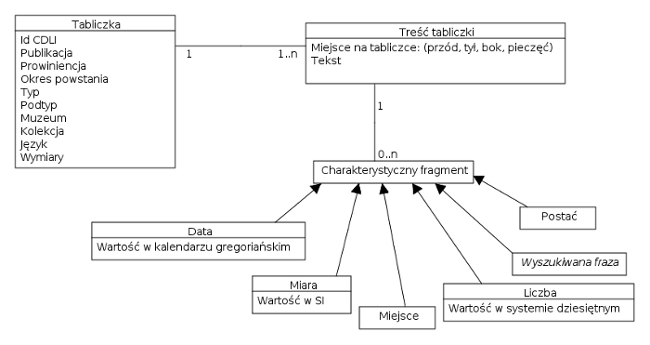
\includegraphics[width=500px]{diagramy/Model-dziedziny.png}
Głównym pojęciem jest tabliczka. Ma ona swoje metadane i treść. Tabliczka jest rozumiana dwojako - jako fizyczna tabliczka gliniana
zapisana klinami lub jako tabliczka w formie cyfrowej zapisana odczytami. Może ona zawierać elementy znaczące takie jak imię jakiejś 
osoby, liczba, jednostka (np. przy opisywaniu wypłat), miejsce, data, imię bóstwa. Część tych elementów da się przetłumaczyć na 
współczesny język (np. jednostki przeliczyć na SI, datę na datę liczbową BC). Gliniane tabliczki są zapisywane z różnych stron 
(od góry, z przodu, z tyłu itp). Poza tym zawierają pieczęcie - fragmenty tekstu po prostu odbijane na tabliczce (coś jak nasza
pieczątka). 

Sumerolodzy rozpoznają tabliczki po publikacjach - wiedzą mniej więcej o co chodzi jak widzą publikację.

Odczyty zawarte w cyfrowym zapisie tabliczki są wariantem tłumaczenia z klinów. W cyfrowej wersji nie ma klinów, stąd też możliwe
są pomyłki w tłumaczeniach, które ciężko zweryfikować. Są też uszkodzone fragmenty, które zostały cyfrowo zapisane w najróżniejszej
formie (np. po niemiecku ``Tutaj miałem problem, ale chyba powinno być <<xxx>>'' (-; )
\chapter{Definicja języka TQL}
\section{Gramatyka}
\subsection{Struktura leksykalna}

\subsubsection*{String}
Literał \nonterminal{String}\ ma postać
\terminal{"}$x$\terminal{"}, gdzie $x$ jest dowolnym ciągiem znaków
poza \terminal{"}\ niepoprzedzonymi \verb6\6.


\subsubsection*{Słowo Od Litery}
Literał \nonterminal{Słowo Od Litery} to ciąg liter, cyfr oraz znaków  {\tt - \_ '}, zaczynający się od litery,
z wyjątkiem słów kluczowych.



\subsubsection*{Słowo Od Liczby}
Literał \nonterminal{Słowo Od Liczby} to ciąg liter, cyfr oraz znaków  {\tt - \_ '}, zaczynający się od cyfry.



\subsection{Słowa kluczowe}
\begin{tabular}{lll}
{\reserved{as}} &{\reserved{define}} &{\reserved{in}} \\
{\reserved{search}} & & \\
\end{tabular}\\

\subsection{Znaki specjalne}
\begin{tabular}{lll}
{\symb{$\backslash$n}} &{\symb{:}} &{\symb{{$+$}}} \\
{\symb{/}} &{\symb{{$-$}{$-$}}} &{\symb{*}} \\
{\symb{(}} &{\symb{)}} & \\
\end{tabular}\\

\subsection{Komentarze}
W chwili obecnej język nie zawiera komentarzy.

\subsection{Struktura syntaktyczna języka}
Nieterminale są pomiędzy $\langle$ a $\rangle$. 
Symbole  {\arrow}  (produkcja),  {\delimit}  (lub) 
i {\emptyP} (pusta reguła) należą do notacji BNF. 
Wszystkie pozostałe symbole to terminale.\\

\begin{tabular}{lll}
{\nonterminal{Zapytanie Złożone}} & {\arrow}  &{\nonterminal{Lista Zapytań}}  \\
\end{tabular}\\

\begin{tabular}{lll}
{\nonterminal{Zapytanie}} & {\arrow}  &{\nonterminal{Lista Linii Zapytania}} {\nonterminal{Lista Pustych Linii}}  \\
 & {\delimit}  &{\terminal{define}} {\terminal{$\backslash$n}} {\nonterminal{Zapytanie}} {\terminal{as}} {\nonterminal{Nazwa}} {\nonterminal{Lista Pustych Linii}}  \\
 & {\delimit}  &{\terminal{search}} {\terminal{$\backslash$n}} {\nonterminal{Zapytanie}} {\terminal{in}} {\nonterminal{Nazwa}} {\nonterminal{Lista Pustych Linii}}  \\
 & {\delimit}  &{\nonterminal{Lista Pustych Linii}}  \\
\end{tabular}\\

\begin{tabular}{lll}
{\nonterminal{Linia Zapytania}} & {\arrow}  &{\nonterminal{Identyfikator}} {\terminal{:}} {\nonterminal{Wyrażenie}}  \\
\end{tabular}\\

\begin{tabular}{lll}
{\nonterminal{Wyrażenie}} & {\arrow}  &{\nonterminal{Wyrażenie}} {\terminal{{$+$}}} {\nonterminal{Wyrażenie1}}  \\
 & {\delimit}  &{\nonterminal{Wyrażenie}} {\terminal{/}} {\nonterminal{Wyrażenie1}}  \\
 & {\delimit}  &{\nonterminal{Wyrażenie1}}  \\
\end{tabular}\\

\begin{tabular}{lll}
{\nonterminal{Wyrażenie1}} & {\arrow}  &{\terminal{{$-$}{$-$}}} {\nonterminal{Wyrażenie1}}  \\
 & {\delimit}  &{\nonterminal{Wyrażenie2}}  \\
\end{tabular}\\

\begin{tabular}{lll}
{\nonterminal{Wyrażenie2}} & {\arrow}  &{\nonterminal{Tekst}} {\terminal{*}} {\nonterminal{Tekst}}  \\
 & {\delimit}  &{\nonterminal{Tekst}} {\terminal{*}}  \\
 & {\delimit}  &{\terminal{*}} {\nonterminal{Tekst}}  \\
 & {\delimit}  &{\nonterminal{Tekst}}  \\
 & {\delimit}  &{\terminal{(}} {\nonterminal{Wyrażenie}} {\terminal{)}}  \\
\end{tabular}\\

\begin{tabular}{lll}
{\nonterminal{Lista Zapytań}} & {\arrow}  &{\nonterminal{Zapytanie}}  \\
 & {\delimit}  &{\nonterminal{Zapytanie}} {\nonterminal{Lista Zapytań}}  \\
\end{tabular}\\

\begin{tabular}{lll}
{\nonterminal{Lista Linii Zapytania}} & {\arrow}  &{\nonterminal{Linia Zapytania}} {\terminal{$\backslash$n}}  \\
 & {\delimit}  &{\nonterminal{Linia Zapytania}} {\terminal{$\backslash$n}} {\nonterminal{Lista Linii Zapytania}}  \\
\end{tabular}\\

\begin{tabular}{lll}
{\nonterminal{Pusta Linia}} & {\arrow}  &{\terminal{$\backslash$n}}  \\
\end{tabular}\\

\begin{tabular}{lll}
{\nonterminal{Lista Pustych Linii}} & {\arrow}  &{\emptyP} \\
 & {\delimit}  &{\nonterminal{Pusta Linia}} {\nonterminal{Lista Pustych Linii}}  \\
\end{tabular}\\

\begin{tabular}{lll}
{\nonterminal{Tekst}} & {\arrow}  &{\nonterminal{String}}  \\
 & {\delimit}  &{\nonterminal{Słowo}}  \\
\end{tabular}\\


\begin{tabular}{lll}
{\nonterminal{Słowo}} & {\arrow}  &{\nonterminal{Słowo Od Litery}}  \\
 & {\delimit}  &{\nonterminal{Słowo Od Liczby}}  \\
\end{tabular}\\

\begin{tabular}{lll}
{\nonterminal{Identyfikator}} & {\arrow}  &{\nonterminal{Słowo Od Litery}}  \\
\end{tabular}\\

\begin{tabular}{lll}
{\nonterminal{Nazwa}} & {\arrow}  &{\nonterminal{String}}  \\
\end{tabular}\\


\chapter{Implementacja}
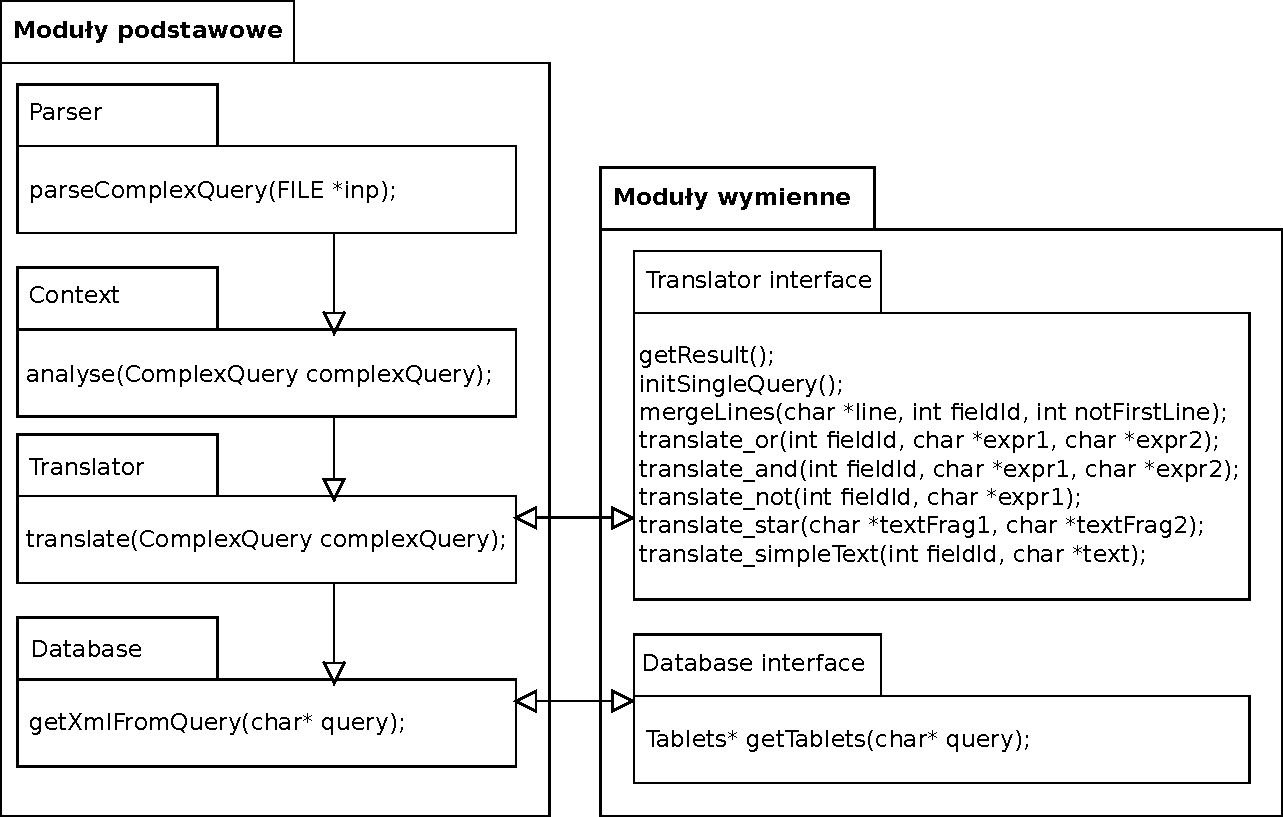
\includegraphics[width=500px]{diagramy/pakiety.pdf}
Implementacja składa się z dwóch części - zależnej i niezależnej od struktury danych. 
\section{Moduły podstawowe}

\subsection{Parser}
Parser został utworzony za pomocą narzędzia BNFC. Następnie został zmodyfikowany ręcznie: nazwy stałych oznaczających symbole, 
dodanie tablicy symboli (stringów), uporządkowanie kodu, zmiana niektórych struktur danych. Na parser składają się następujące pliki:
\begin{itemize}
 \item Parser.c
\item Parser.h
\item TQL.y % tłumaczony na Parser.c
\item TQL.l % tłumaczony na Lexer.c
\end{itemize}



\subsection{Analizator kontekstowy}
\begin{itemize}
 \item sprawdza, czy to co jest po lewej w linii zapytania jest nazwą pola.
\item upraszcza zapytania - z zapytania złożonego (wywołanie search in) tworzy jedno zapytanie proste
\item wypełnia strukturę danych
\end{itemize}
Składa się z następujących plików:
\begin{itemize}
 \item Context.c
 \item Context.h
\end{itemize}

\subsection{Translator}
Zadaniem translatora jest przetłumaczenie struktury (drzewa składni abstrakcyjnej) jaka powstała na zapytanie w danym języku. 
Składa się z następujących plików:
\begin {itemize}
 \item Translator.c
 \item Translator.h
 \item Translator\_config.h
 \item Translator\_config.c (implementacja interfejsu z Translator\_config.h, zależny od wyboru bazy danych itp)
\end {itemize}

To jak poszczególne elementy są tłumaczone zależy od pliku Translator\_config.c (interfejs jest w Translator\_config.h). Plik Translator.c 
przechodzi całą strukturę i od czasu do czasu wywołuje funkcję z Translator\_config.

\subsection{Baza}
Moduł bazy jest odpowiedzialny za wywołanie przetłumaczonego zapytania i przekazanie wyniku w określonej formie - w tym momencie xml.
Składa się z następujących plików:
\begin {itemize}
 \item Database.c
 \item Database.h
 \item Database\_config.h
 \item Database\_config.c (implementacja interfejsu z Database\_conf.h, zależny od wyboru bazy danych itp)
\end {itemize}
Wywołuje funkcję z Database\_config.h, jako parametr podaje treść zapytania, funkcja zwraca wypełnioną strukturę danych Tablets.


\begin{verbatim}
typedef struct{    
    char* id;
    char* id_cdli;
    char* publication;
    char* measurements;
    char* year;
    char* provenience;
    char* period;
    char* genre;
    char* subgenre;
    char* collection;
    char* text;
    Tags *tags; //miejsca gdzie w tekście są wyniki wyszukiwania
} Tablet;

typedef struct{
    int size;
    Tablet *tabs;
} Tablets;
\end{verbatim}

Następnie tłumaczy otrzymaną strukturę na xml-a.

\subsection{Pliki pomocnicze}
Tablica symboli (stringów):
\begin{itemize}
 \item symbols.c
\item symbols.h
\end{itemize}
Obsługa błędów:
\begin{itemize}
 \item Err.c
\item Err.h
\end{itemize}
Definicja struktur danych:
\begin{itemize}
 \item Absyn.c
\item Absyn.h
\end{itemize}
Moduł do dzielenia tekstu wg. separatora, implementacja funkcji explode z php (pobrane z internetu):
\begin{itemize}
 \item Cexplode.c
 \item Cexplode.h
\end{itemize}


\section{Moduły wymienne}
Pliki zależne od wyboru konkretnej bazy danych to:
\begin{itemize}
 \item Translator\_config.c
\item Database\_config.c
\end{itemize}
Ich interfejs jest wspólny dla wszystkich baz danych.

\subsection{Baza PostgreSQL}
\subsubsection{Diagram encji}
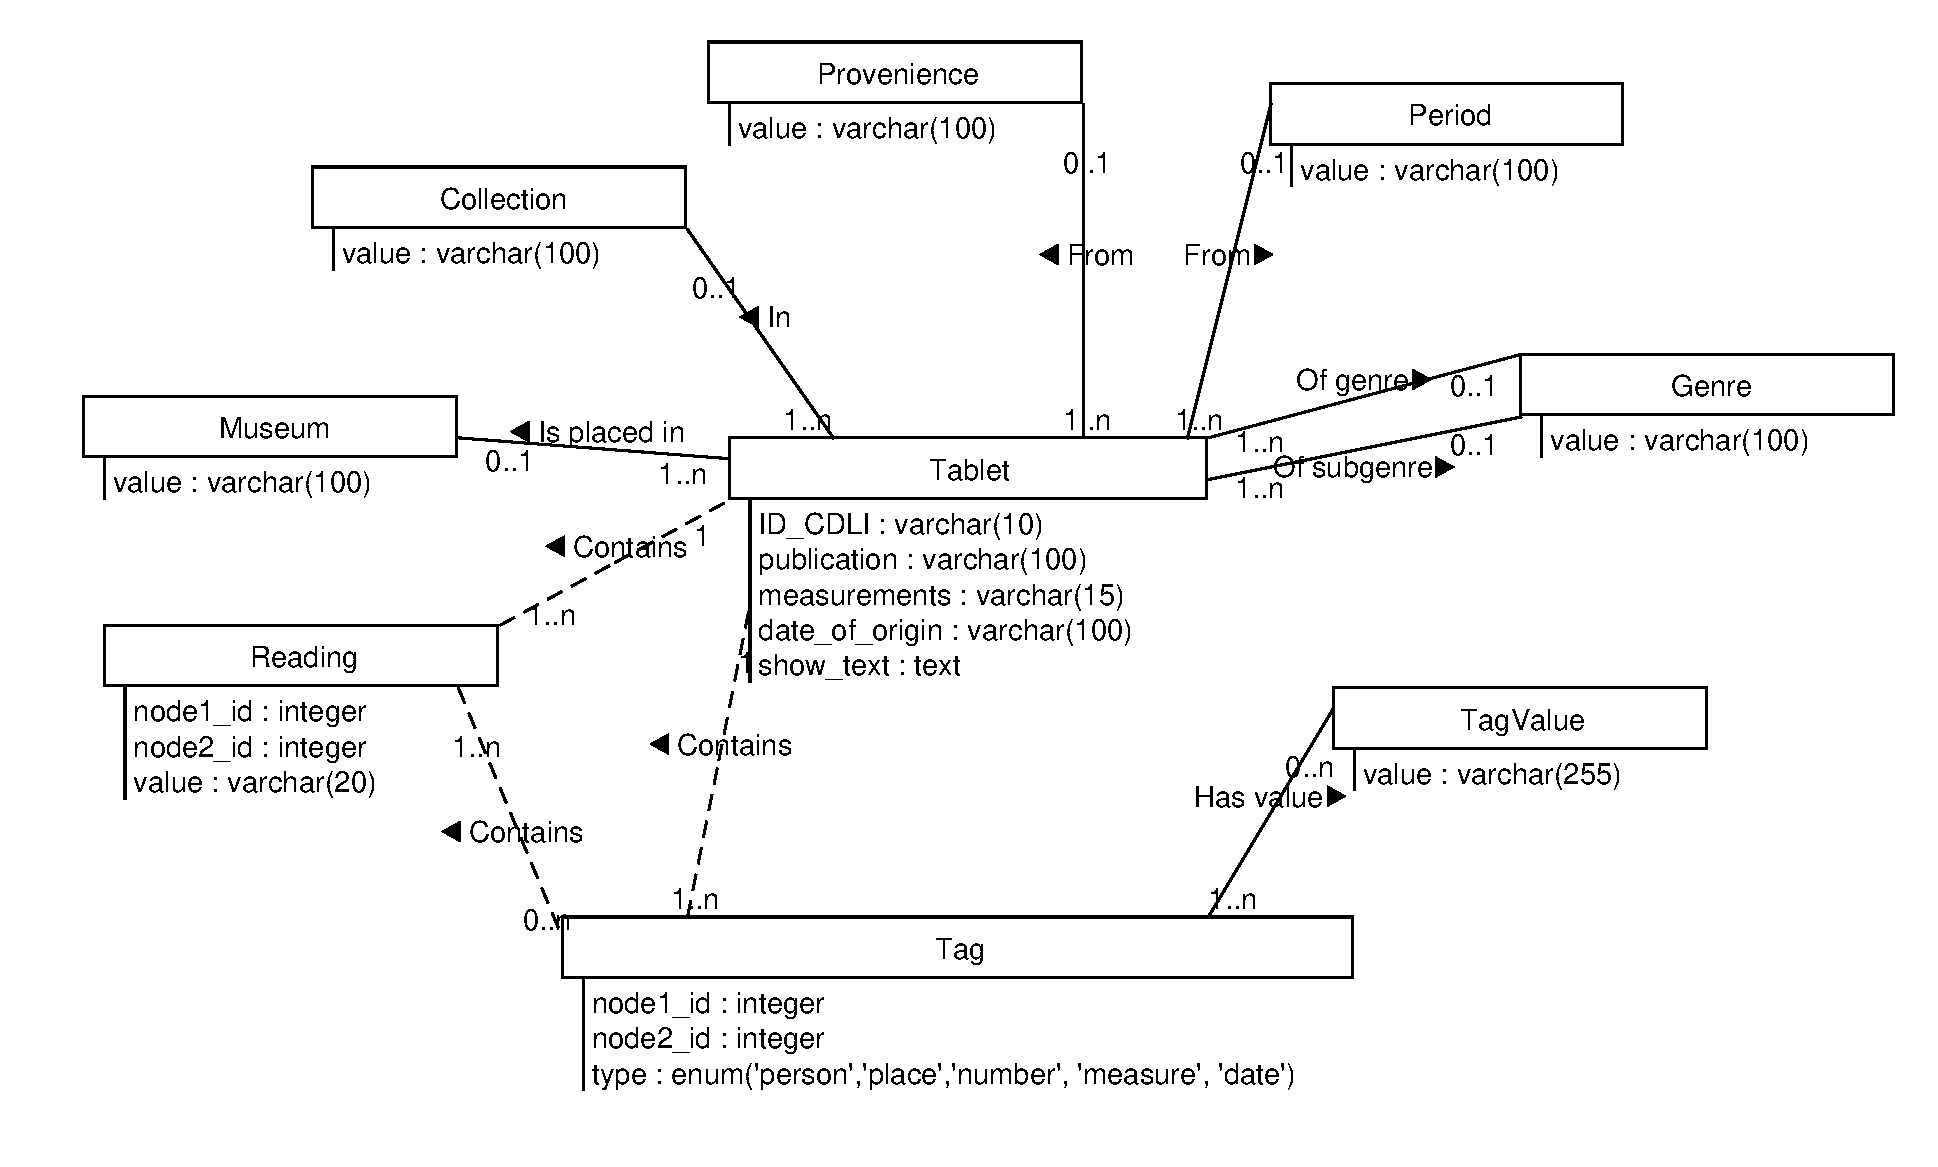
\includegraphics[width=500px]{diagramy/diagram-encji-maly.pdf}
\subsubsection{Translator\_config}
Dostaje poszczególne fragmenty drzewa struktury zapytania i tłumaczy je na SQL. Przetłumaczone fragmenty zbiera do buforów (select, from, where), które następnie odpowiednio skleja.
Każde proste zapytanie jest tłumaczone na jednego selecta; jak jest kilka prostych zapytań to są sklejane UNION.

\subsubsection{Tłumaczenie konstrukcji}
\begin{longtable}{|p{3in}|p{3in}|}
\hline
{\bf Konstrukcja} & {\bf Tłumaczenie na SQL}\\
\hline
\endhead
provenience: wartosc & \begin{description}
     \item[From] 
     \item[Where] p.value LIKE 'wartosc'
     \end{description}\\
\hline
publication: wartosc & 
\begin{description}
     \item[From]
     \item[Where] t.publication LIKE 'wartosc'
     \end{description}\\
\hline
period: wartosc & 
\begin{description}
     \item[From]
     \item[Where] pd.value LIKE 'wartosc'
     \end{description}\\
\hline
year: wartosc & \begin{description}
     \item[From]
     \item[Where] t.origin\_date LIKE 'wartosc'
     \end{description}\\
\hline
genre: wartosc & \begin{description}
     \item[From]
     \item[Where] g1.value LIKE 'wartosc' OR g2.value LIKE 'wartosc'
     \end{description}\\
\hline
cdli\_id: wartosc & \begin{description}
     \item[From]
     \item[Where] t.cdli\_id LIKE 'wartosc'
     \end{description}
\\
\hline
text: wartosc & \begin{description}
     \item[From]
     \item[Where] 
     \end{description}
\\
\hline
\end{longtable}


% \begin{array}{ll}
% x & x \\
% \textbf{Konstrukcja} & \textbf{Tłumaczenie na sql}\\
% \end{array}



\subsubsection{Database\_config}
Odpowiada za wywołanie zapytania na konkretnej bazie. Korzysta z pliku database.conf, który zawiera dane dostępu do bazy. Korzysta z biblioteki libpq-fe.h do postgresa. Zwrócony wynik zapisuje do struktury Tablets.

\subsection{Baza XML}

%\chapter{Dokumentacja użytkowa i opis implementacji}\label{r:impl}

\chapter{Podsumowanie}


\appendix



\begin{thebibliography}{99}
\addcontentsline{toc}{chapter}{Bibliografia}

%\bibitem[Bea65]{beaman} Juliusz Beaman, \textit{Morbidity of the Jolly
 %   function}, Mathematica Absurdica, 117 (1965) 338--9.

\end{thebibliography}

\end{document}


%%% Local Variables:
%%% mode: latex
%%% TeX-master: t
%%% coding: latin-2
%%% End:
